%----------------------------------------------------------------------------
%PACKAGES AND OTHER DOCUMENT CONFIGURATIONS
%----------------------------------------------------------------------------
\documentclass[paper=a4, fontsize=11pt]{scrartcl} % A4 paper and 11pt font size

\usepackage[T1]{fontenc} % Use 8-bit encoding that has 256 glyphs
\usepackage{fourier} % Use the Adobe Utopia font for the document - comment this line to return to the LaTeX default
\usepackage[english]{babel} % English language/hyphenation
\usepackage{amsmath,amsfonts,amsthm} % Math packages

\usepackage{graphicx} % Used for including graphics
\usepackage{caption}
\usepackage{subcaption}
\usepackage{listings}

\usepackage{sectsty} % Allows customizing section commands
\allsectionsfont{\centering \normalfont\scshape} % Make all sections centered, the default font and small caps

\usepackage{fancyhdr} % Custom headers and footers

\usepackage{cite}
\bibliographystyle{plain}

\pagestyle{fancyplain} % Makes all pages in the document conform to the custom headers and footers
\fancyhead{} % No page header - if you want one, create it in the same way as the footers below
\fancyfoot[L]{} % Empty left footer
\fancyfoot[C]{} % Empty center footer
\fancyfoot[R]{\thepage} % Page numbering for right footer
\renewcommand{\headrulewidth}{0pt} % Remove header underlines
\renewcommand{\footrulewidth}{0pt} % Remove footer underlines
\setlength{\headheight}{13.6pt} % Customize the height of the header

\numberwithin{equation}{section} % Number equations within sections (i.e. 1.1, 1.2, 2.1, 2.2 instead of 1, 2, 3, 4)
\numberwithin{figure}{section} % Number figures within sections (i.e. 1.1, 1.2, 2.1, 2.2 instead of 1, 2, 3, 4)
\numberwithin{table}{section} % Number tables within sections (i.e. 1.1, 1.2, 2.1, 2.2 instead of 1, 2, 3, 4)

\setlength\parindent{0pt} % Removes all indentation from paragraphs - comment this line for an assignment with lots of text

% Definitions of theorem environments
\newtheorem{theorem}{Theorem}[section]
\newtheorem{lemma}[theorem]{Lemma}
\newtheorem{proposition}[theorem]{Proposition}
\newtheorem{corollary}[theorem]{Corollary}

%\newenvironment{proof}[1][Proof]{\begin{trivlist}
%\item[\hskip \labelsep {\bfseries #1}]}{\end{trivlist}}
\newenvironment{definition}[1][Definition]{\begin{trivlist}
\item[\hskip \labelsep {\bfseries #1}]}{\end{trivlist}}
\newenvironment{example}[1][Example]{\begin{trivlist}
\item[\hskip \labelsep {\bfseries #1}]}{\end{trivlist}}
\newenvironment{remark}[1][Remark]{\begin{trivlist}
\item[\hskip \labelsep {\bfseries #1}]}{\end{trivlist}}

% Indents for paragraphs
\usepackage{indentfirst}
\setlength{\parindent}{1cm} % Default is 15pt.

%----------------------------------------------------------------------------
%	TITLE SECTION
%----------------------------------------------------------------------------

\newcommand{\horrule}[1]{\rule{\linewidth}{#1}} % Create horizontal rule command with 1 argument of height

\title{
\normalfont \normalsize
\textsc{King Abdullah University of Science and Technology\\
        Division of Mathematical and Computer Sciences and Engineering\\
        Design and Analysis of Algorithms} \\ [25pt] % Your university, school and/or department name(s)
\horrule{0.5pt} \\[0.4cm] % Thin top horizontal rule
\Large Midterm Project Report\\
\huge Diverse Approaches to Exact Pattern Matching
\horrule{2pt} \\[0.5cm] % Thick bottom horizontal rule
}

\author{Affara, Lama\\
        Almansour, Durrah\\
        Al-Shedivat, Maruan\\
        Chen, Gui\\
        Fujii, Chisato\\
        Rapakoulia, Trisevgeni}


\date{\normalsize\today} % Today's date or a custom date


\begin{document}

\begin{titlepage}
\maketitle
\thispagestyle{empty}
\clearpage
\end{titlepage}

\section{Introduction}
\par Pattern matching remains to this day an extensively studied problem. The exponential growth of computing and data collection has increased the need for a more efficient solution to this problem. Pattern matching is applied in a wide range of disciplines such as database queries, text editors, two dimensional meshes, bioinformatics, music content retrieval, spell checkers, digital libraries, search engines, etc.

\par One optimal algorithm that can be applied to all such applications which include different data formats has not been established. Therefore, the intention to test the performance of three different algorithms: Boyer-Moore, Aho-Corasick, and Suffix-tree algorithms. In this report, we present theoretical analysis and comparison of the time complexities of the above three algorithms. Further, we will perform an experimental comparison applying them on texts, patterns, and alphabets of various types and lengths.

\par Pattern matching can be defined as follows~\cite{intro}: \textit{Given a text T of length n and a pattern P of length k over some alphabet $\Sigma$, where n > k, the exact pattern matching problem consists of finding all occurrences z of the pattern P in the text T}. For example, let p = aba and t = abaababa over alphabet $\Sigma$ = \{a,b\}. As illustrated in Figure~\ref{fig:matching}, three occurrences of the considered pattern appear in the text, at locations 1, 4, and 6. A variety of algorithms have been developed for exact pattern matching, the most famous of which are presented in Figure~\ref{fig:algorithms}.

\begin{figure}[h!]
\centering
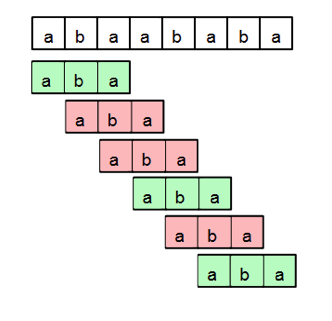
\includegraphics[width=0.37\textwidth]{figures/matching.png}
\caption{Pattern matching instance.}
\label{fig:matching}
\end{figure}

\begin{figure}[h!]
\centering
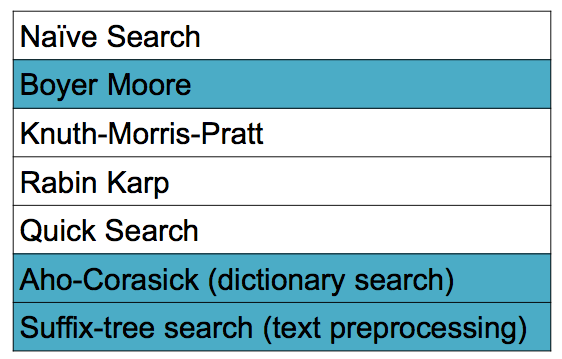
\includegraphics[width=0.4\textwidth]{figures/algorithms.png}
\caption{Algorithms for exact pattern matching.}
\label{fig:algorithms}
\end{figure}

\newpage
\section{Boyer-Moore Algorithm}
\par Boyer Moore algorithm \cite{bm_fast} searches for all the occurrences of the pattern in the text. It is in some way similar to the na\"ive search algorithm. Initially, it aligns the first character in P with the first character in T. The algorithm then compares characters between P and T sequentially from right to left. Once a mismatch occurs, a shift rule is applied thus moving the pattern by $s\ge 1$. The algorithm is basically divided into two stages: preprocessing and searching. There are two different preprocessing approaches in the literature: \textit{Bad Character Rule} and \textit{Good Suffix Tree}~\cite{bm_tbc}. We decided to choose the Bad Character Rule due to its simplicity and applicability to our dataset. In the following sections, we describe the two stages of the algorithm.

\begin{figure}[h!]
\centering
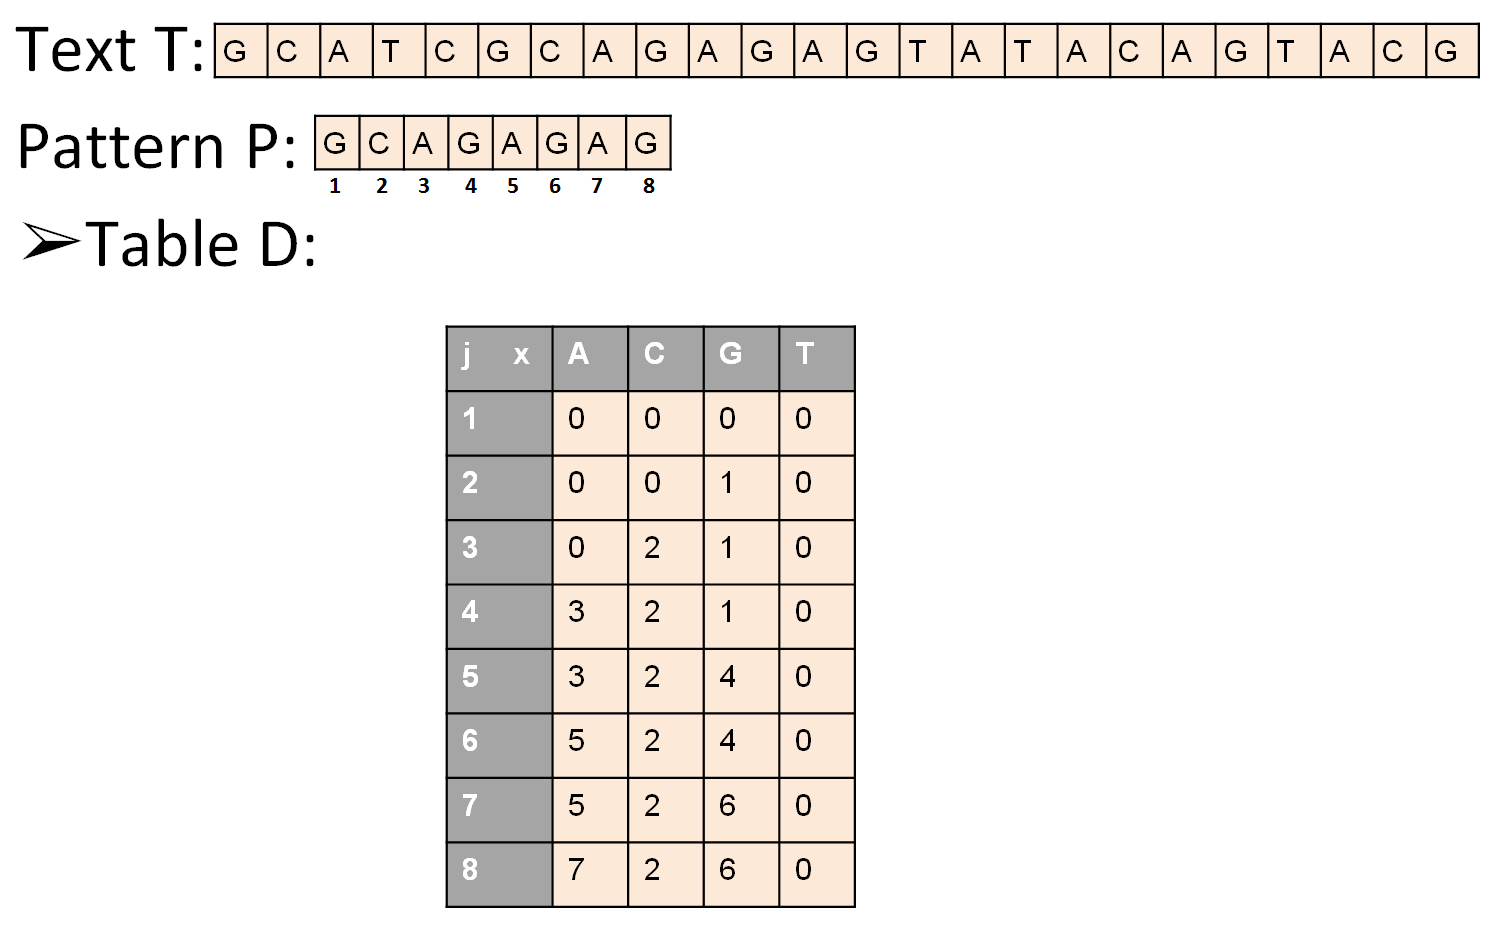
\includegraphics[width=\textwidth]{figures/Example_Table.png}
\caption{Table of preprocessing phase.}
\label{fig:table}
\end{figure}

\subsection{Preprocessing Stage}
\par In the preprocessing stage, the algorithm makes use of the alphabet $\Sigma$ and the pattern P. A two dimensional table D is constructed by processing the pattern according to the available alphabet. D is of size $k\times|\Sigma|$ where for each mismatch index in P, the position of rightmost occurrence of a character in $\Sigma$ is stored. Figure~\ref{fig:table} shows an example of the table stored by processing the pattern $GCAGAGAG$ based on the DNA $alphabet=\{A,C,G,T\}$. Starting from the last row corresponding to a mismatch occurring at position $i=k$ in $P$, $i=8$ for this example, the algorithm scans $P$ to find the rightmost index of the given character. In the below example, the last occurrence of A before position 8 is 7, $G$ is 6, $C$ is 2, and $T$ is 0. It is important to note here that if a character does not exist in the pattern, its position in the table is always 0. The algorithm iterates from $i=k$ to 1. If the mismatch occurs in position $i-1$, the algorithm updates only the value for the specific character placed in this position, A for this example, and all the other values remain the same as $D[i,x]$. The last occurrence of A before position 7 is 5, while $G$, $C$, and T stay the same.


\subsection{Searching Phase}
\par In the searching phase, the algorithm shifts the pattern and sequentially matches it with the aligned text. Starting from the rightmost character in P, the algorithm checks the aligned character in T. If the pair of characters are matched, it sequentially continues to check the next left character. If a mismatch occurs at the position $j$ in $P$, the algorithm shifts $P$ according to the mismatched character $x$ in the text. For example, if at the position $j$, if the text contains a character that is not found in $P$, the pattern is shifted by $j$. However, if the mismatched character is found in $P$, the pattern is shifted by $j-i$, where $i$ corresponds to the rightmost occurrence of this character in $P$. The index $i$ of the last occurrence is retrieved from table $D$ ($i=D[j,x]$ where $x$ is the character in the text). Figure \ref{fig:search} shows the searching phase for the example shown in the previous section. The pseudocode of Boyer-Moore algorithm is shown below.

\begin{lstlisting}
Algoritm: BMMatch(T, P):
Input: Text T (n characters) and pattern P (k characters)
Output: List I of indexes of occurences of P in T

D=Preprocess(P)
l=k
j=k
z=0
repeat
    if P[j] = T[l] then
        if j = 0 then
            I[z]=l;
	    z=z+1
        else {check next character}
            l = l - 1
            j = j - 1
    else { P[j] <> T[l] shift the pattern}
        x=T[l]
	i=D[j,x]
	l = l + k - j - 1 {reset l to position of P in T}
        l=l+ j - i
        j =k
until l > n
return "There is no substring of T matching P."
\end{lstlisting}

\par In the searching phase, the algorithm needs shift the pattern and sequentially match it with the aligned text. Starting from the rightmost character in $P$, the algorithm checks the aligned character in $T$. If the pair of characters are matching, it sequentially continues the check to the next left character. If a mismatch occurs at position $j$ in $P$, the algorithm needs to shift P according to the mismatched character in the text. For example, if at position $j$, the text contains a character that is not found in $P$, the pattern should be shifted by $j$. However, if the mismatched character is found in $P$, the pattern should be shifted by $j-i$, where $i$ corresponds to the rightmost occurrence of this character in $P$. The index i of the last occurrence is retrieved from table $D$ and $i=D[j,x]$ where $x$ is the character in the text. Figure \ref{fig:search} shows the searching phase for the example shown in the previous section.

\begin{figure}[h!]
\centering
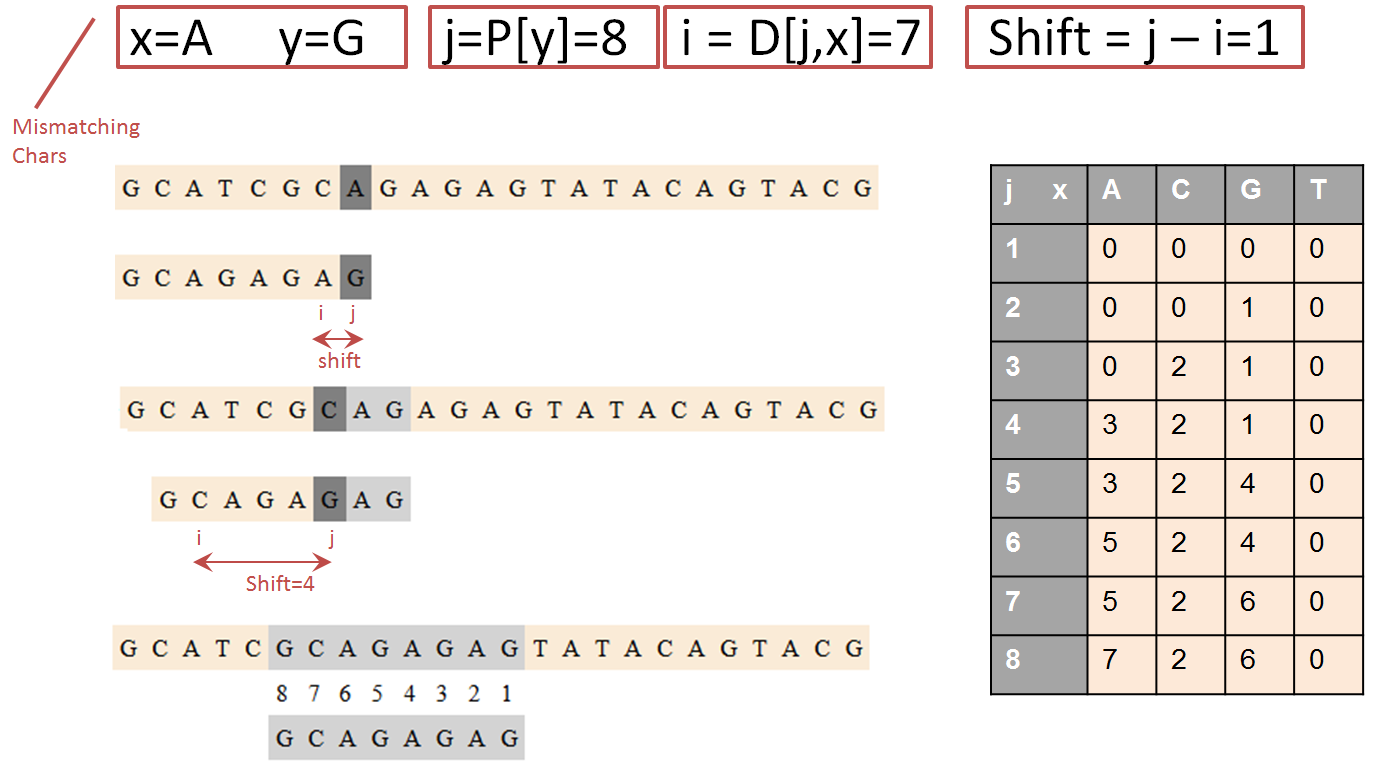
\includegraphics[width=0.8\textwidth]{figures/searching_phase.png}
\caption{Searching Phase.}
\label{fig:search}
\end{figure}

\subsection{Complexity}
\par In this section we show the time complexity for both the preprocessing and searching phases of the algorithm. For the preprocessing stage, a table of $k\times|\Sigma|$ is stored in memory, so the space complexity is $O(k\times|\Sigma|)$. Initially, the first row is initialized to zeros. At each step, one value is updated in the table and the rest of the values are copied from the row before it. So at each step, $i<k$, $|\Sigma|$ operations are done. Thus, the preprocessing time complexity is $O(k\times|\Sigma|)$. For the searching phase, the text $T$ is compared to pattern $P$ from right to left. The worst time occurs when the shifts are only one character at a time and the algorithm would be similar to naive search with a complexity of $O(k\times n)$. However, the shifts employed by this algorithm allow it to have a sublinear complexity especially in the case of large alphabet and random strings.

\newpage
\section{Aho-Corasick algorithm}
\par Aho-Corasick algorithm \cite{aho} is a generalization of the Knuth-Morris-Pratt algorithm. It takes one or more patterns (a dictionary) to be searched in the text. Suppose, the total length of all patterns is $k$. Then, the algorithm pre-processes the patterns and constructs a Deterministic Finite Automaton (DFA) \cite{hopcroft} in $O(k)$ time. The obtained DFA processes a text and reports pattern occurrences in linear time too -- $O(n + z)$, where $z$ is the number of occurrences to be found. The $O(z)$ term is for that we assume that we can report all the occurrences in linear time. The example of the DFA is given in the figure \ref{dfa}.

\begin{figure}[h!]
\centering
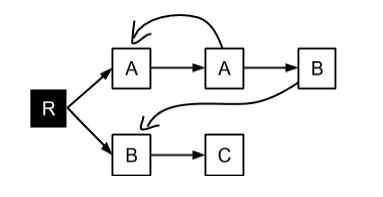
\includegraphics[width=0.8\textwidth]{figures/Example_DFA.png}
\caption{A DFA representing a set of patterns {AAB, BC}.}
\label{dfa}
\end{figure}

\subsection{Construction of DFA}
\label{sec:dfa_const}
\par Each node consists of a character is represents, a flag signifying whether or not it is a dictionary node, and a set of the patterns it represents. A dictionary node is a special kind of node which marks the end of a pattern or more, and those patterns are stored in the set of patterns it represents.

\begin{enumerate}
\item Forward Edge: Connecting a node representing character at position i in pattern p to the one representing the character at position i+1 in the same pattern.
\item Reverse Edge: Connecting a node to another node representing the same value in a higher level (closer to the root) provided they have the same value parents, which is insured during the building.
\end{enumerate}

\subsubsection{Setting Up the Nodes and Forward Edges}
\begin{enumerate}
\item First a root node is created and set to be the current node. The first pattern is selecter and a pointer is set to point to the first character in it.

\item If the current node does not have a forward edge to a node representing the current character, then such a node is created and a forward edge connects the current node to it. The new node becomes the the current node.

\item If the current node has a forward edge to a node representing the current character, then that node becomes the current node.

\item The pointer in the pattern moves to the next character

\item If there are no more characters in the pattern, mark the node as dictionary node with the corresponding pattern, then select the next pattern in the list and make the pointer point to the first character in it. Set the current node to the root and repeat steps 2 through 5 until there are no more patterns in the list.
\end{enumerate}

\subsubsection{Setting Up the Reverse Edges}
Expanding a node means dequeuing it and enqueuing its child nodes.
\begin{enumerate}
\item Start from the node and expand it into its children, put the child nodes into a queue.

\item Point the reverse edges of the children of the root back to the root.

\item Expand the node at the front of the queue.

\item For each node x of the children of the newly expanded node do the following:

\begin{enumerate}
    \item Set the parent of the newly expanded node as the current node.

    \item If the current node has a child node with the same value as node x, point x's reverse edge to that child, and if this child node happens to be a dictionary node for pattern p, mark node x as a dictionary of the same patter p. 
    \item If this child node does not have the same value as node x, check that it is the root, and if so, point x's reverse edge to it. Otherwise go to the node pointed to by the reverse edge of the current node set it as the current node and repeat 4.b and 4.c.
\end{enumerate}
\end{enumerate}

\subsubsection{Searching}
The search algorithm outputs any patterns it find. Input: string of length n.\\

\begin{enumerate}
\item set the current node to root node
\item for every character c of the input string:
\begin{enumerate}
\item if the current node has a forward edge pointing to a node x with the value of c, set the current node to be node x. 
\item if there is not such a forward edge, then if the current node is not the root, set the node pointed to by the reverse edge as the current node and repeat step 2.a. if the current node is the root, skip the rest of this step and step 2.c,   
\item If the current node is a dictionary node, output the patterns it represents.
\end{enumerate}
\end{enumerate}

\subsection{Theoretical Analysis}
For our analysis we will use the following notations: $k$ is the total length of all patterns, $n$ is the number of characters in input string, and $z$ is the number of pattern occurrences in the text.

\subsubsection{Preprocessing}
\par Preprocessing is done in two steps:
First, a Deterministic Finite Automaton (DFA) is built according to the patterns as described in the previous section. Setting up nodes and creating forward edges requires $k$ time.
Second, traversing the DFA to add the reverse edges involves going forward $k$ times and going up the reverse edges of a number of nodes. This number is bounded by the $k$, the total length of patterns since in the worst case a node at the end of each pattern will point back to the root. This gives a total of $2k$ for this step. Hence, the preprocessing yields a runtime of  $3*k = O(k)$. 

\subsubsection{Searching}
\par Each character in the input text must be compared to the content of a node once, therefore a minimum of n computations is needed for comparisons, while outputting a pattern set of a dictionary node takes constant time. However, since pattern sets are output whenever they are found in the text, then the number of times the algorithm outputs a pattern, must be taken into consideration. The worst case is when patterns are found at virtually every position of the input string. For example, let the set of patterns be $\left\{a, a^2,\dots, a^m\right\}$ where m is the length of the longest pattern, and let the text by $a^n$, such that $a^i$ is i a's. This can also be represented by alphabet in $|\Sigma|$ = $\left\{a\right\}$.

\begin{enumerate}
  \item When $n = 1$, $A(1)$ outputs $\left\{a\right\}$, the result of the first node.
  \item When $n = 2$, $A(2) = \left\{a\right\} + \left\{a, a^2\right\} = A(1) + \left\{a, a^2\right\}$.
  \item Assume that when $n = i$, then $A(i) =  \left\{a\right\} + \left\{a, a^2\right\} + \dots + \left\{a, a^2, ..., a^i\right\}$.
  \item Then when $n = i+1$, $A(i+1) = \left\{a\right\} + \left\{a, a^2\right\} + \dots + \left\{a, a^2, ..., a^i\right\} + \left\{a, a^2, ..., a^i, a^(i+1)\right\}$ which can be rewritten as  $A(i+1) = A(i) + \left\{a, a^2, ..., a^i, a^{i+1}\right\}$.
\end{enumerate}
This shows that in the worst case, the number of pattern occurrences in the text, denoted as z, is the dominating factor in the time complexity, yielding $O(n+z)$. In the worst case the term $z$ grows similarly to the sum of running time of applying Naive Search on each pattern in the pattern set, which will be $k\times n$.

\newpage
\section{Suffix-tree Pattern Matching}
\par As the third part of our comparative study, we consider a pattern matching algorithm that relies on so called \textit{suffix tree} data structure. Suffix tree is a well known data structure which is commonly used in industrial and scientific applications of pattern matching today. Being a concise representation of a text composed over a finite alphabet, suffix tree, or more general suffix automaton, is a common way to compress large amounts of textual information, and it is widely used also in databases. In our study, we will perform tests of suffix tree based pattern matching algorithm, and compare it against the aforementioned Boyer-More and Aho-Corasick algorithms trying to get an insight on when should one chose either of these algorithms.

\par Below, we will introduce first \textit{suffix trie} -- an auxillary data structure -- which we will enhance into suffix tree. Along this way, we will show that suffix tree construction algorithm is a linear time algorithm, and that suffix tree is a linear-memory data structure. We will follow the Ukkonen's construction algorithm~\cite{ukkonen1995line}. Suffix tree construction is the preprocessing step for the pattern matching algorithm. We will describe how to use a suffix tree of a text to find out if a pattern matches the text, and will show that procedure also takes pattern length linear time.

\subsection{Suffix Trie}
\par Being able to consider suffix tries, and following~\cite{ukkonen1995line}, we first introduce the notations. Let text T be a string $T = t_1 t_2 \dots t_n$ over an alphabet $\Sigma$; $T_i = t_i \dots t_n$ where $1 \leq i \leq n+1$ is a suffix of the text; lets also assume that $T_{n+1} = \varepsilon$, i.e. the empty suffix. Lets denote the set of all the suffixes of the text T by $\sigma(T)$. We name the following set of objects a \textit{suffix trie} of a text T:

\begin{equation}
STrie(T) = \left\{Q \cup \{\perp\}, root, F, g, f \right\}
\end{equation}
which is a deterministic finite-state automaton (DFA) that has a tree-shaped transition graph representing the trie for $\sigma(T)$. It is augmented with so called \textit{suffix function} $f$ and with an auxiliary state $\perp$. In the presented notations, the set $Q$ is the set of all the states of $STrie(T)$, which could be put into one-to-one correspondence with the substrings of $T$, i.e. with all such $x$ that $T = a\ x\ v$, where $a$ is some prefix of $T$, and $v$ is some suffix of $T$. The initial state $root$ corresponds to the empty string $\varepsilon$, and the set of final states $F$ corresponds to all the suffixes $\sigma(T)$. Latin characters with bars will denote states; characters without bars will denote symbols or some sequences of symbols from the alphabet $\Sigma$; $\varepsilon$ will denote the empty string. Finally, the transition function $g$ is defined as $g(\bar{x}, a) = \bar{y}$ for all $\bar{x}, \bar{y} \in Q$ such that $y = xa$, where $a \in \Sigma$; $g(\perp, a) = root$ for all $a \in \Sigma$.

\par Now, the suffix function $f$ is defined for each state $\bar{x} \in Q$ as follows: If $\bar{x}$ is not $root$, then there exist $a \in \Sigma$ such that $x = az$; we set $f(\bar{x}) = \bar{z}$. We also define $f$ for the $root$ as $f(root) = \perp$.

\subsubsection{Suffix Trie Online Construction}
\par To online construct a suffix trie by reading a text $T$ from left to right, symbol by symbol, we should notice the following. Suppose, we have already read some prefix of the text $T^i = t_1 \dots t_i$, and have already constructed a $STrie(T^i)$. Now, we read the next symbol $t_{i+1}$ from the text, and we need to add it to the structure and obtain $STrie(T^{i+1})$. One can notice, that all the new suffixes of $T^{i+1}$ could be obtained by concatenation of $t_{i+1}$ symbol to all the previous suffixes, i.e.

$$
\sigma(T^{i+1}) = \sigma(T^i)t_i \cup \varepsilon.
$$

\par By construction, the $STrie(T^i)$ accepts $\sigma(T^i)$, and we want to make it accept $\sigma(T^{i+1})$. For achieving this, we need to add $t_{i+1}$ transitions to all the $r \in F_i$ which don't have such. By doing this, we will properly update our transition function $g_i$ to $g_{i+1}$, and also we will get final states $F_i$ updated to $F_{i+1}$.

\par Also, we should update the suffix function $f_i$ up to $f_{i+1}$, such that for every $\bar{r} \in F_{i+1}$ the new suffix function $f_{i+1}(\bar{r}) = \bar{s}$, for which $r = as$, where $a \in \Sigma$. In order to do such an update, we notice that if $r \in F_i$, then there exists such $0 \le j \le i$, such that $r = f_i^j(\overline{t_1...t_i})$. This means that the suffix function connects all the final states in the $STrie(F_i)$ into a single path. We denote this path as the \textit{boundary path}.

\subsubsection{Suffix Trie Analysis}
\par So, the new suffix function $f_{i+1}$ should connect all the new final states $F_{i+1}$ and form a new boundary path. To achieve this, we can traverse all the $F_i$ states along the current boundary path, and make updates for every state on this path, adding a suffix link where it is necessary and adding a transition for a new symbol $t_{i+1}$ where it is necessary. Finally, it was shown in the original paper~\cite{ukkonen1995line} that while traversing the boundary path, if we encountered a state $\bar{z}$ that does have a transition $t_{i+1}$, there is no need to further continue traversing, since all of the further suffix successors of the state $\bar{z}$ are up-to-date and have both the right suffix links and also the right transitions $t_{i+1}$. Finally, the algorithm is going to be as it follows.

\begin{enumerate}
  \item Start from the state $\overline{t_1 t_2 \dots t_i}$ (the whole prefix preprocessed up to now).
  \item If there is no transition from the current state for symbol $t_{i+1}$, create a new state for such a transition. Memorize the newly created state.
  \item Follow the suffix link from the current state and again perform step (2).
  \item Create a suffix link from the last created state (on step 3) for transition on symbol $t_{i+1}$, to the state created right before that (on step 2).
  \item Repeat steps (2), (3) and (4) until we find that the current state has a transition on $t_{i+1}$.
\end{enumerate}

\begin{figure}[h!]
\centering
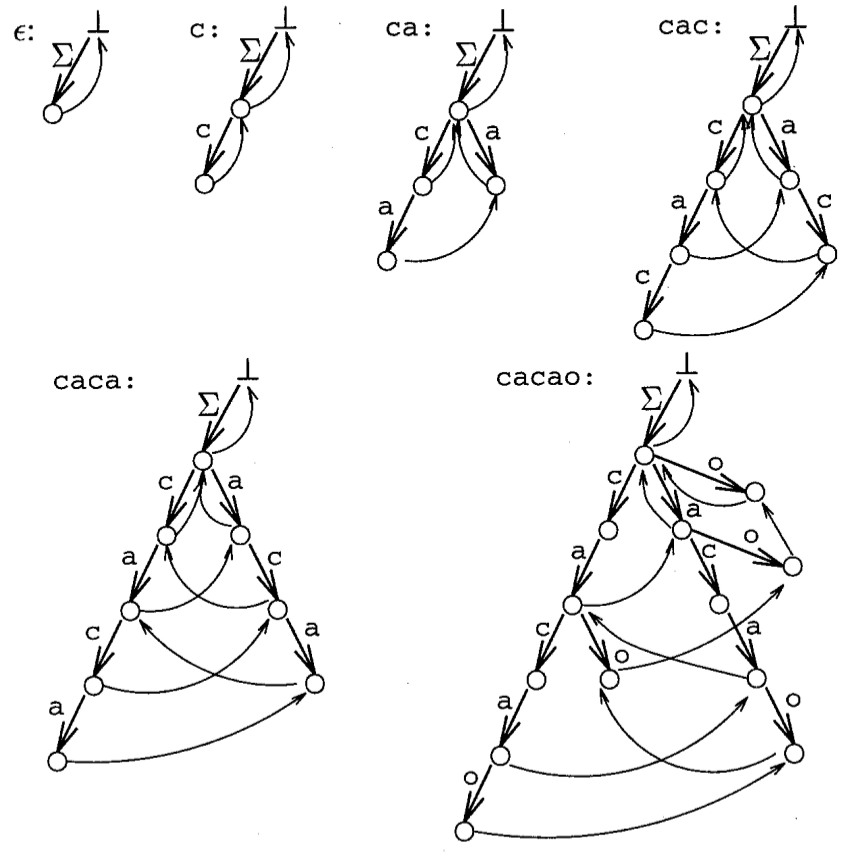
\includegraphics[width=0.75\textwidth]{figures/suffix-trie-eg.png}
\caption{An example of building a suffix trie for the string "cacao". We start from the empty string, and the suffix trie augmented DFA consists of only $root$ and $\perp$ states at this stage. Then we add letter by letter the whole text. For each letter, we perform the above mentioned 5-step iterative algorithm to update the transition and suffix functions $g$ and $f$.}
\label{fig:siffix-trie}
\end{figure}

\par An example of how this algorithm works is presented in figure~\ref{fig:siffix-trie}. The algorithm obviously does a constant number of operations each of its iterations, and, in the worst case, it should visit all the nodes of the suffix trie $STrie(T^i)$ to update it up to $STrie(T^{i+1})$. So, it is optimal in the sense that its time complexity is proportional to the size of its end result $STrie(T)$. On the other hand, the size of $STrie(T)$ can be quadratic in $n = |T|$. To overcome this issue, we introduce the so called \textit{suffix tree} structure which is based on suffix trie, but is more concise and takes less memory and time to be built.

\subsection{Suffix Tree}
\par In order to introduce suffix tree structure, first, we reduce the set of states $Q \cup \{\perp\}$ described above to the set $Q' \cup \{\perp\}$ -- the set of so called \textit{explicit states} -- which includes only the \textit{branching states} -- the states that have two or more children, i.e. from which there are two or more transitions -- and the \textit{leaves} -- the states that don't have any transitions. The other states $Q \ Q'$ are called \textit{implicit}. By definition, we also include $root$ state into the set of explicit states $Q'$ regardless its branching.

\par Since we reduced the set $Q$ to $Q'$, if we want to go from one explicit state to another, we have to spell out not only one symbol, but, in general, a substring $w$ of the text $T$. So, second, we have to generalize the transition function. The new function $g'$ will take as arguments an explicit state and a substring $w$, and it will return another explicit state: $g'(\bar{r}, w) = \bar{s}$. To save memory, we also will represent substrings $w$ as two pointers to $T$: left pointer $k$ and right pointer $p$. So, the new transition function can be written as $g'(\bar{r},(k,p)) = \bar{s}$.

\par Finally, we need to introduce a new suffix function compatible with the set $Q'$ of only explicit states. So, we say that the new suffix function $f'$ is defined for all the explicit states, and it returns an explicit state: $f'(\bar{x}) = \bar{y}$, such that $x = ay$, where $a \in \Sigma$ \footnote{If $\bar{x}$ is an explicit state, then $f'(\bar{x})$ is explicit too, since they share the same suffixes, and hence the same transitions.}.

Now, we denote the following structure as suffix tree:

\begin{equation}
STree(T) = \left\{ Q' \cup \{\perp\}, root, g', f' \right\}.
\end{equation}

\par Since, we keep only the explicit states in the suffix tree, but we need to have anyway access to all the states including implicit ones, we introduce so called \textit{reference pair} $(\bar s, w)$ which consists of an explicit state $\bar s$ and a substring $w$ of the text $T$. Using such pairs, we can easily refer to all the explicit as well as implicit states of the $STree(T)$. We name a reference pair \textit{canonical}, if the state $\bar s$ of the pair has the maximum possible level in the tree, and hence $w$ is the shortest possible.

\subsubsection{Suffix Tree Analysis}
\par Suffix tree has two components: the tree itself and the string $T$. It is of linear size in $n \equiv |T|$ because $Q'$ has at most $n$ leaves (at most one leaf for each non-empty suffix), and therefore $Q'$ has to contain at most $n - 1$ branching states (when $n > 1$) \footnote{To understand that a tree with branching factor $b >= 2$ and with $n$ leafs, has the total number of nodes equal to $O(n)$, we can see that the number of all the nodes can be upper bounded with $1 + 2 + 2^2 + \dots + 2^d$, where $d = \log_2n$, and hence the number of nodes will be $O(n)$. If we do a little more strict derivations, we can show that in fact the number of all the leafs in such a tree is upper bounded by $2n - 1$, where $n$ is the number of leaves.}. Now, since the alphabet is finite, the number of transitions will be also bounded, and it will be in our case equal to $O(n)$. The number of suffix links we have to store will be less than or equal to the number of all the explicit states, i.e. $O(n)$. So, this proves that the constructed suffix tree is a linear in memory data structure.

\subsubsection[Suffix Tree Online Construction Algorithm]{Suffix Tree Online Construction Algorithm\footnote{This part is the most complex piece of the analysis. We tried to simplify our considerations and make them as succinct as it is possible, yet we recommend to refer to the original paper~\cite{ukkonen1995line} for any additional subtle details omitted in the following discussion.}}
\par Now, we need to enhance the proposed above algorithm for a suffix trie construction to make it able to construct a suffix tree. First, we introduce some additional notations, and a lemma without a proof (the proof is essential and completely based on the consideration of two different cases of the algorithm for an $STrie$ construction). Lets denote all the states corresponding to suffixes in the currently processed prefix $T^i$ by $\bar s_1, \bar s_2, \dots, \bar s_i$ where $\bar s_h = \overline{t_1 t_2 \dots t_{i - h + 1}}$.

\begin{lemma}
\label{lemma:active-end-point}
Algorithm 1 adds to $STrie( T^i)$ a $t_{i+1}$-transition for each of the states $\bar{s}_h$,
$1 < h < j'$, such that, for $1 < h < j$, the new transition expands an old branch of
the trie that ends at leaf $\bar{s}_h$, and, for $j < h < j'$, the new transition initiates a new branch from $\bar{s}_h$. Algorithm 1 does not create any other transitions.
\end{lemma}

\par Further, we call the state $\bar{s}_j$ the \textit{active point} and the state $\bar{s}_{j'}$ the \textit{end point} of $STrie(T^i)$. According to this lemma, there are two important segments of the boundary path: the segment in which we add new transitions to the traversed leaves ($1 < h < j'$, right before active point), and the segment in which we split the states and increase their branching factor ($j \le h < j'$, between the active point and the end point).

\par Now, we go back to $STree(T^i)$. The updates with no splits we can just update the transition, adding $t_{i+1}$ symbol: For example we have a transition to a leaf (we also call it an \textit{open transition}) $g'(\bar{s}, (k, i)) = \bar{r}$ where the pointer $i$ points to the last symbol of the previous text prefix $T^i$. So, in this case we need to update the transition and make it $g'(\bar{s}, (k, i+1)) = \bar{r}$. Now, again, the right pointer $i+1$ now points right to the end of the current text prefix $T^{i+1}$. We can use this property and all the leaf transitions we can represent as $g'(\bar{s}, (k, \infty)) = \bar{r}$, denoting the pointer to the last symbol of the current prefix as $\infty$. Such notation automatically updates all the states $s_h$ in $STree(T^{i+1})$ before the active point ($1 < h < j'$).

\begin{figure}[h!]
\centering
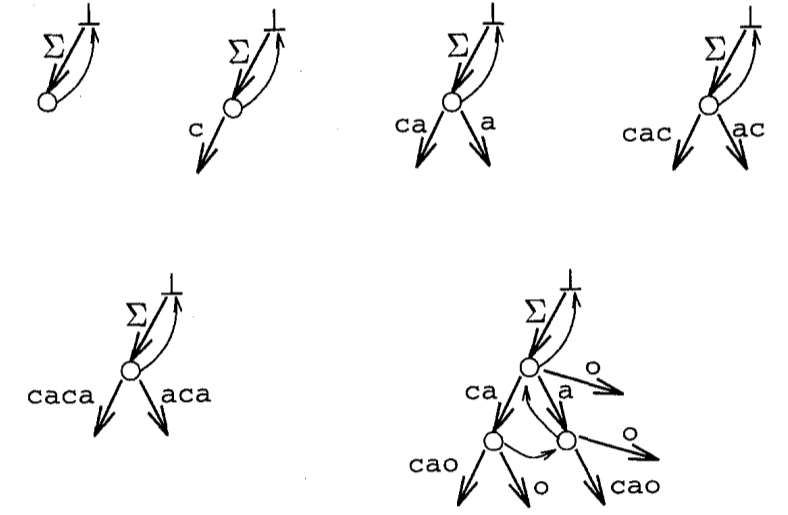
\includegraphics[width=0.8\textwidth]{figures/suffix-tree-eg.png}
\caption{An example of building a suffix tree for the string "cacao". Notice that the suffix tree is much more concise than the suffix trie for the same example string.}
\label{fig:siffix-tree}
\end{figure}

\par Finally, we need to consider the procedure of adding transitions to states $\bar s_h$ along the boundary path between the active point and the end point ($j \le h < j'$) splitting the nodes. We start from the state $\bar s_j$ (the active point). Lets denote the \textit{canonical reference pair} of the active point by $(\bar s, w)$, which is by definition (see lemma~\ref{lemma:active-end-point}) is the same as $(\bar s, (k, i-1))$. We first check if the end point coincides with the canonical point. If yes, we are done. Otherwise, we should create a new branch, splitting the current state if it is implicit. The newly created transition will be $g'(\bar s_h, (i, \infty)) = \bar s'_h$ where $\bar s'_h$ is a new leaf. Also, if $\bar s_h$ was implicit and became explicit by splitting, a new suffix function link $f'(s_h)$ should be added. Then we advance the construction to the next state $\bar s_{h+1}$.

\par Before we start working with the next state, we need to make sure that its reference pair is canonical. For this purpose, we use procedure \textit{canonize}, which updates the reference pair of the current state to the canonical representation \footnote{To see how exactly \textit{canonize} procedure works (along with some additional subtle moments of the algorithm), please refer to the original paper~\cite{ukkonen1995line}.}. So, the final procedure that updates $STree(T^i)$ to the $STree(T^{i+1})$ is as following:

\begin{enumerate}
  \item Let the current point be the active point,
  \item canonize the current point,
  \item create a new transition from the current point to a new state,
  \item if current point is not root, create a suffix link from the current point,
  \item if necessary check and split the current state,
  \item repeat steps (2)--(5) until the current point is not equal to the end point.
\end{enumerate}

\subsubsection{Construction Algorithm Analysis}
\noindent The main theorem that was stated in~\cite{ukkonen1995line} is

\begin{theorem}
\label{theorem:suffix-tree-theorem}
The proposed algorithm constructs the suffix tree $STree(T)$ for a string $T = t_1 t_2 \dots t_n$ on-line in time O(n).
\end{theorem}

\par The idea of the proof is the following. We divide the runtime of the algorithm into two components: (1) the total time for the procedure \textit{canonize}, (2) the repeated traversals along the boundary path from the active point to the end point doing splits along this way where it is necessary. In~\cite{ukkonen1995line} it was shown that both \textit{canonize} and repeated traversals consist of constant time operations (checks, state splits, etc.), the number of which is O(n)\footnote{To be precise, it was shown, that the number of constant time steps done during traversals $\le 2n$, and it is $O(n)$ with some constant around 2 for the \textit{canonize}.}. So, the total time of the construction algorithm will be linear.

\subsubsection{Pattern Matching using Suffix Trees}
\par Suppose, we are given a pattern $P$ and a text $T$, the pattern matching problem is to find all occurrences of $P$ in $T$. Let $|P| = k$ and $|T| = n$. Typically, $n >> k$. Moreover, $T$ remains fixed in many applications and the query is repeated for many different patterns. For example, $T$ could be a text document and $P$ could represent a word search. Or, $T$ could be an entire database of DNA sequences and $P$ denotes a substring of a query sequence for homology (similarity) search. Thus, it is beneficial to preprocess the text $T$ so that queries can be answered as efficiently as possible.

\par The pattern matching problem can be solved in optimal $O(k+z)$ time using $STree(T)$, where z is the number of occurrences of $P$ in $T$. Suppose $P$ occurs in $T$ starting from position $i$. Then, $P$ is a prefix of suffix in $T$. It follows that $P$ matches the path from root to leaf labelled $i$ in $STree$. This property results in the following simple algorithm: Start from the root of $STree$ and follow the path matching characters in $P$, until $P$ is completely matched or a mismatch occurs. If $P$ is not fully matched, it does not occur in $T$. Otherwise, each leaf in the subtree below the matching position gives an occurrence of $P$. The positions can be enumerated by traversing the subtree in time proportional to the size of the subtree. As the number of leaves in the subtree is $z$, this takes $O(z)$ time. If only one occurrence is of interest, the suffix tree can be preprocessed in $O(n)$ time such that each internal node contains the label of one of the leaves in its subtree. Thus, the problem of whether $P$ occurs in $T$ or the problem of finding one occurrence can be answered in $O(k)$ time.

\subsubsection{Example of Matching a Pattern with a Suffix Tree}
\par Suppose that we have a suffix tree of a text $banana\$$, as shown in the Figure~\ref{fig:suffix-tree-ex}. The length of the text is 6, so it has 7 leaves. Each leaf represents a suffix of the text. From figure~\ref{fig:suffix-tree-ex}, there are 7 suffixes, which are $\$$, $a\$$, $na\$$, $ana\$$, $nana\$$, $anana\$$, $banana\$$. At the end of the text we should use so called \textit{sentinel sign} -- a symbol which isn't present in the alphabet $\Sigma$. This is done to make all the text suffix states explicit leaves.

\begin{figure}
\centering
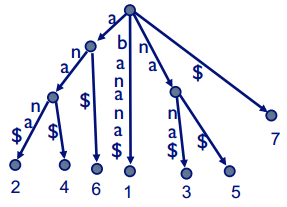
\includegraphics[width=3.5in]{figures/suffixtree.png}
\caption{Suffix tree of a text: $banana$}
\label{fig:suffix-tree-ex}
\end{figure}

\par For a given pattern $Q$, the algorithm will follow a unique path down from root of $T$ according to characters in $Q$. If all characters of $Q$ is found to be a prefix of such a path, then return the labels of some leaves below this path. If there a mismatch occurs, then return ``no match found''.

\par For example, for a given pattern $Q = \{nan\}$ and a given pattern $Q = \{anab\}$, the algorithm works as shown in the Figure~\ref{fig:suffix-tree-matching-ex}. Basically, for every character in a given pattern, it requires $O(1)$ time to compare with the character in the suffix tree. Therefore, it needs $k*O(1)$, namely, $O(k)$ time to report a matching, where $k$ is the length of a given pattern. Assume that there are $z$ matchings, therefore the leaves of the sub-tree that below the end of the path is equal to $z$. Thus it requires $O(z)$ time to report all the leaves that below the end of the path. Therefore, the total time complexity to report all the matchings is $O(k+z)$, where $k$ denotes the length of the pattern and $z$ denotes the number of the matchings.

\begin{figure}
\begin{center}
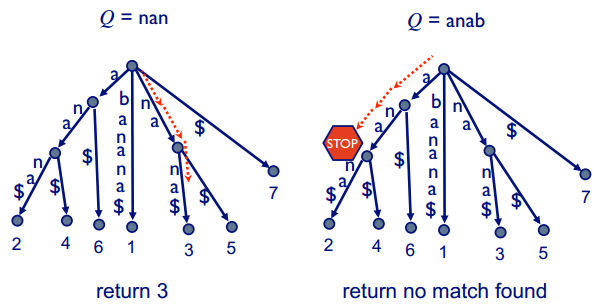
\includegraphics[width=5.5in]{figures/example.png}
\caption{Examples of pattern $nan$ and $anab$}
\label{fig:suffix-tree-matching-ex}
\end{center}
\end{figure}

\subsubsection{Suffix Tree Based Pattern Matching Algorithm Complexity}
As it was shown above, algorithm takes linear time to preprocess the text and build the suffix tree of the text, i.e. preprocessing takes $O(n)$ time. Pattern matching is also linear, and it takes $O(k + z)$ time in the above introduced notation.

\newpage
\section{Dataset}
\par We will apply these algorithms on an available dataset of DNA sequences and natural language text, to find specific sequence motifs in the former, and words and phrases in the latter. With regards to the biological dataset, we selected the DNA sequence of human chromosome 1 in fasta format as a searching test. The DNA alphabet consists of four elements, $\Sigma = \{A,\ C,\ G,\ T\}$, that represent  the four nitrogenous bases. We also chose three different patterns for our experimental measurements. As for the natural language data set, we will search for specific phrases of varying lengths. We will compare the performance in the two data sets to highlight the effect of the size of the alphabet and pattern length. Applying the algorithms on these datasets will show practical results on the analytical complexities that we examined and the difference in performance of the three above mentioned algorithms on the tested domains of application.


Both natural language text and DNA input text were formatted as $.txt$ and any special characters were removed.

\section{Experiment}
\par In order to observe the effect of parameters n and k in runtime complexity, we vary each parameter while other parameters are fixed. This is applied to both the text and the pattern. We first fixed the length of text n and vary the length of pattern k from 1 to 100. Then we fix the length of the pattern k and vary the length of the text to from 1 with increments of 1000 char length. We obtain the time taken for running each algorithm in above conditions and plot the graph showing the effect of n and k.

For the DNA dataset, the fixed length text of 50000 was used for the input test. The pattern length was varied from the length of one character (i.e $A$) to the length of 100 characters $TCTGG...TCGAA$. 

\section{Discussion}
\par Each algorithm has a one time preprocessing cost. Aho-Corasick algorithm has linear search cost to the length of the input text and the occurrences of the patterns in the input text. When the alphabet in $|\Sigma|$ has a single character, the term $z$ in Aho-Corasick grows similarly to the sum of running time of applying Na\"ive Search on each pattern in the pattern set, which will be $k\times n$, resulting in the worst case running time for Aho-Corasick. However, such a small alphabet has a positive effect on Boyer-Moore, resulting in a smaller preprocessing time.

\par Suffix tree algorithm appears to be a complete opposite to Aho-Corasick, since it preprocesses the whole text, and if the length of the text is much bigger than the cumulative length of the set of patterns, then it takes much more time to construct the suffix tree automaton, than to construct Aho-Corasick's automaton. Though, for each pattern to be processed it doesn't filter the whole text to match the pattern to it, which is crucial in applications where the text is static, and there is a stream of patterns to be processes (e.g. search engine).

\par Also, suffix tree algorithm has a few hidden constants behind its linearity in time of the preprocessing and the searching steps. These constants are very sensitive to the size of the alphabet, to the frequency of each of the symbols in the alphabet, and hence the experimental study is needed to completely understand the algorithm's behavior under different conditions.

\begin{table}[h!]
\centering
\begin{tabular}{| l | l | l | l |}
	\hline
	& Boyer-Moore & Aho Corasick & Suffix Tree \\
	\hline
	Pre-processing & $O(|\Sigma|)$ & $O(k)$ & $O(n)$ \\
	\hline
	Searching & $O(k\times n)$ & $O(n + z)$ & $O(k + z)$ \\
	\hline
\end{tabular}
\caption{Comparative table of preprocessing and searching time complexities.}
\end{table}


\newpage
\bibliography{references}
%\nocite{*}

\end{document}
